\documentclass{article}

\usepackage[utf8]{inputenc} % allow utf-8 input
\usepackage[T1]{fontenc}    % use 8-bit T1 fonts
\usepackage[hidelinks]{hyperref}       % hyperlinks
\usepackage{url}            % simple URL typesetting
\usepackage{booktabs}       % professional-quality tables
\usepackage{amsmath,amssymb,amsthm}
\usepackage{amsfonts}       % blackboard math symbols
\usepackage{nicefrac}       % compact symbols for 1/2, etc.
\usepackage{makecell}
\usepackage{microtype}      % microtypography
\usepackage{mathrsfs}
\usepackage{graphicx}
\usepackage{doi}
\usepackage{acronym}
\usepackage{listings}
\usepackage{tikz}
\usepackage[dvipsnames]{xcolor}

\usetikzlibrary{trees}

\newcommand{\R}{\mathbb{R}}

\title{TODO}

\begin{document}

\twocolumn

\section*{}

\begin{figure}
    \centering
    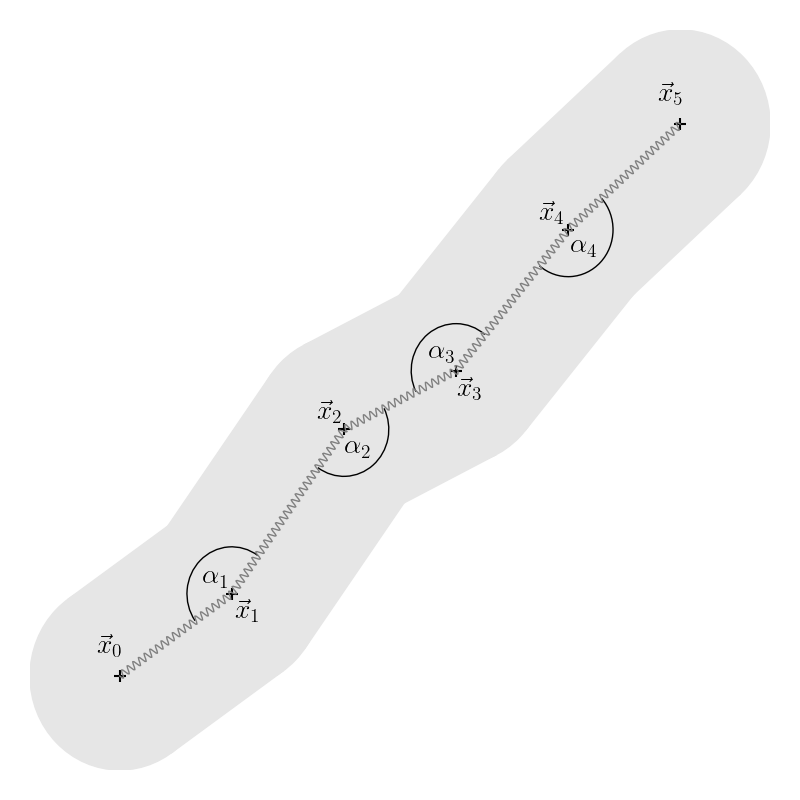
\includegraphics[width=0.5\textwidth]{figures/mechanics.png}
    \caption{TODO}
\end{figure}

\begin{itemize}
    \item Represent bacterial rods as collection of vertices $\vec{x}_i$ where $i=1..N$ and
        $\vec{x}_i\in\R^d$ with $d=2,3$
    \item Many bacteria $j=1..M$.
    \item Gives us tensor $\eta_{i,j}^k\in \R^{N\times M\times d}$
\end{itemize}

\bibliographystyle{IEEEtran}
\bibliography{references}

\end{document}
